\documentclass{beamer}
\usetheme{Madrid}
\usepackage[spanish]{babel}
\usecolortheme{default}
\usepackage{emoji}
\usepackage[most]{tcolorbox}
\usepackage{listings}
\usepackage{xcolor}
\usepackage{colortbl}
\usepackage{graphicx}
\usepackage{algorithm}
\usepackage{algpseudocode}
\usepackage{float}
\usepackage{mathtools}
\usepackage{hyperref}
\makeatletter
\newcases{centercases}{\quad}
  {\hfil$\m@th\displaystyle{##}$\hfil}
  {$\m@th\displaystyle{##}$\hfil}{\lbrace}{.}
\makeatother

\usepackage{comment}
\usepackage{minted}

\usepackage{tikz}
\usetikzlibrary{arrows.meta,positioning}
\usetikzlibrary{calc}

% Define Python syntax highlighting
\lstdefinestyle{pythonstyle}{
    language=Python,
    basicstyle=\ttfamily\tiny,
    keywordstyle=\color{blue},
    commentstyle=\color{gray},
    stringstyle=\color{red},
    numbers=left,
    numberstyle=\tiny\color{gray},
    stepnumber=1,
    showstringspaces=false,
    frame=none,
    breaklines=true,
    numbersep=4pt, % Reduce space between numbers and text
    xleftmargin=10pt % Reduce left margin for compactness
}






%Information to be included in the title page:
\title[Control de Versiones, CI/CD] %optional
{Control de Versiones, CI/CD}

\subtitle{MISUM}

\author[José A.] % (optional, for multiple authors)
{José Antonio Hernández López\inst{1}}

\institute[UMU] % (optional)
{
  \inst{1}%
  Departamento de Informática y Sistemas\\
  Universidad de Murcia
}

%\date[VLC 2021] % (optional)
%{Very Large Conference, April 2021}



%\logo{\includegraphics[height=1cm]{overleaf-logo}}
\begin{document}

\frame{\titlepage}

\begin{frame}
\frametitle{Índice}
\tableofcontents
\end{frame}

\section{Sistemas de control de versiones}

\subsection{Definición y tipos}

\begin{frame}{Sistemas de control de versiones}

\begin{block}{Definición}
Un sistema de control de versiones (VCS, Version Control System) es una herramienta que permite registrar, gestionar y coordinar los cambios en archivos (normalmente código fuente) a lo largo del tiempo. Son fundamentales en desarrollo de software colaborativo.
\end{block}

\pause

Existen dos tipos:

\begin{itemize}
    \item Sistemas de control de versiones centralizados
    \item Sistemas de control de versiones distribuidos
\end{itemize}

El sistema de control de versiones que más se utiliza es Git. El cual es distribuido.
    
\end{frame}

\begin{frame}{Sistemas de control de versiones centralizados}

\begin{itemize}
    \item Son los primeros que surgen para facilitar el trabajo colaborativo (antes \texttt{archivo.py}, \texttt{archivo\_final.py}, \texttt{archivo\_super\_final.py}, ...)

    \pause

    \item En este modelo, existe un único repositorio central (servidor), que almacena todo el historial del proyecto. Los desarrolladores actúan como clientes: descargan (checkout), modifican en su copia local y luego suben sus cambios (commit) al servidor

    \pause

    
    \item El ejemplo más conocido es Subversion, el cual ya casi no se usa (empresas grandes, organismos públicos y proyectos antiguos)

    \pause

    
    \item ¿Por qué no se usan? Punto único de fallo, poca flexibilidad para ramas y fusiones, requieren conexión permanente, etc.
\end{itemize}

    
\end{frame}

\begin{frame}{Sistemas de control de versiones centralizados}
Fujo de trabajo típico:

\begin{enumerate}
    \item Checkout: los usuarios descargan la última versión desde el servidor.

\item Edición local: trabajan en sus máquinas.

\item Commit: suben sus cambios al servidor central.

\item Update / Merge: si otros usuarios han modificado los mismos archivos, el sistema intenta fusionar los cambios.
\end{enumerate}
\end{frame}

\begin{frame}{Sistemas de control de versiones distribuidos}

\begin{itemize}
    \item Estos sistemas permiten que cada desarrollador tenga \textbf{una copia completa del repositorio} (código + historial + ramas). No dependen de un único servidor para operar: puedes commit, branch y merge en local, y sincronizar después con otros repositorios mediante push/pull

    \pause

    \item \textbf{Operaciones locales}: commit, branch, merge, diff, log no requieren red

    \item \textbf{Sincronización}: intercambio de cambios por push/pull o fetch entre repos internos o remotos

    \item \textbf{Flujos flexibles}: no existe un “servidor único obligatorio”; puedes tener varios remotos

    \item El sistema más famoso y usado es Git
\end{itemize}
    
\end{frame}

\subsection{Git}

\begin{frame}{Git}

\begin{itemize}
    \item Creador: Linus Torvalds (el creador de Linux) en el 2005
    \item El núcleo Linux usaba un sistema propietario (BitKeeper). Al retirarse la licencia, Linus desarrolló Git.
    
\end{itemize}

\begin{figure}
    \centering
    
\includegraphics[width=0.3\linewidth]{linus.png}
\end{figure}
    
\end{frame}

\begin{frame}{Git}

Un repositorio local Git tiene tres zonas:
\begin{itemize}
    \item Working Directory: archivos ''vivos'' en tu carpeta. Si no hay cambios, el estado es el mismo que el último commit (borrador).

    \item Staging Area: zona intermedia donde preparas los cambios que irán en el commit (carpeta donde eliges qué hojas entregar).

    \item Local Repository: historial completo guardado en .git (archivo oficial con todas las versiones entregadas).
\end{itemize}
    
\end{frame}

\begin{frame}{Git}

Cada archivo en Git, puede estar en uno de estos estados:

\begin{itemize}
    \item Untracked:	El archivo no está siendo seguido por Git (nuevo sin git add).
    %\item Tracked:	Git conoce el archivo (fue añadido antes).
    \item Unmodified: El fichero está trackeado por Git y no se ha cambiado desde el último commit.
    \item Modified:	El fichero se ha modificado desde el último commit.
    \item Staged:	Los cambios han sido preparados (git add) para el próximo commit.
    %\item Committed:	Los cambios están guardados en el repositorio local (historial).
\end{itemize}

\begin{figure}
    \centering
    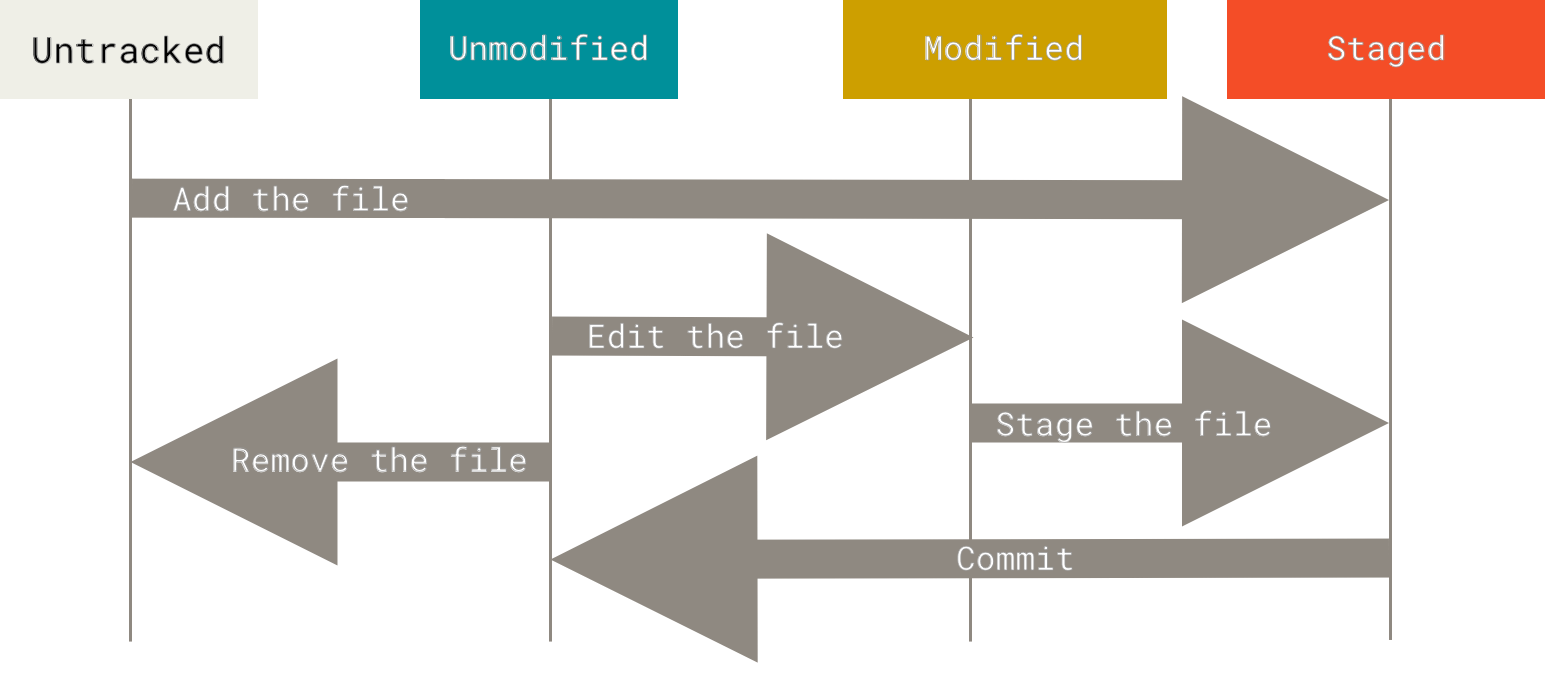
\includegraphics[width=0.5\linewidth]{lifecycle.png}\end{figure}
    
\end{frame}

\begin{frame}{Git: commit}

Cuando se hace un commit (se confirman los cambios con \texttt{git commit}):

\begin{enumerate}
    \item Git toma lo que está en el Staging Area (es decir, los cambios que añadiste con \texttt{git add})

    \item Guarda una ''foto'' completa del proyecto en ese momento en su base de datos interna (.git)

    \item  Crea un objeto \textit{commit} con:

    \begin{itemize}
        \item La foto de los archivos.
        \item La referencia al commit anterior.
        \item Nombre del autor, fecha y mensaje.
        \item Un hash único (ID) que identifica ese commit.
    \end{itemize}


    \item Actualiza la rama actual para que apunte a este nuevo commit.

    \item Limpia el staging area, dejándolo sincronizado.
\end{enumerate}
    
\end{frame}

\begin{frame}{Git: creación de repositorios}

Creación de un repositorio, tenemos dos opciones:

\begin{itemize}
    \item \texttt{cd proyecto} y \texttt{git init}. A partir de ahí se crea un directorio \texttt{.git} que almacenará todos los datos del historial y la configuración de un repositorio de Git
    \item \texttt{git clone <url>} clona un repositorio remoto en un nuevo directorio local, descargando todo su contenido e inicializando la carpeta \texttt{.git} con el historial completo del proyecto.
\end{itemize}
    
\end{frame}

\begin{frame}{Git: comandos}

\begin{table}[h]
\centering
\renewcommand{\arraystretch}{1.3}
\scalebox{0.55}{
\begin{tabular}{|l|p{9cm}|}
\hline
\textbf{Comando} & \textbf{Descripción} \\
\hline
\texttt{git clone url [dir]} & Copiar un repositorio Git para poder añadirle elementos. \\
\hline
\texttt{git add file} & Añadir el contenido del archivo al área de preparación. \\
\hline
\texttt{git commit} & Registrar una instantánea del área de preparación. \\
\hline
\texttt{git status} & Ver el estado de tus archivos en el directorio de trabajo y el área de preparación. \\
\hline
\texttt{git diff} & Mostrar la diferencia entre lo que está preparado y lo que está modificado pero no preparado. \\
\hline
\texttt{git help [command]} & Obtener información de ayuda sobre un comando concreto. \\
\hline
\texttt{git pull} & Ir a buscar (\textit{fetch}) de un repositorio remoto y tratar de fusionar (\textit{merge}) en la rama actual. \\
\hline
\texttt{git push} & Enviar tus nuevas ramas y datos a un repositorio remoto. \\
\hline
\textit{Otros}: \texttt{init, reset, branch, checkout, merge, log, tag} & Otros comandos comunes de Git. \\
\hline
\end{tabular}}
\caption{Comandos básicos de Git}
\end{table}

    
\end{frame}

\begin{frame}{Git: confirmar y deshacer cambios}

\begin{itemize}
    \item La primera vez que pedimos que un archivo sea rastreado, y cada vez
antes de confirmar un archivo, debemos añadirlo al área de staging

\begin{itemize}
    \item \texttt{git add <file\_name>}
    \item \texttt{git add -A} para añadir todos los ficheros modificados
\end{itemize}

    \item Para hacer commit de los cambios en \textit{staged}: 
    
    \texttt{git commit -m ''arreglado bug \#23''}

    \item Para eliminar de la zona de \texttt{stage}:

    \begin{itemize}
        \item \texttt{git reset HEAD -- <filename>} o 
        \item \texttt{git restore --staged <filename>}
    \end{itemize}

    \item Para deshacer los cambios:
    \begin{itemize}
        \item \texttt{git checkout -- <filename>} o 
        \item \texttt{git restore  <filename>}
    \end{itemize}
\end{itemize}
    
\end{frame}

\begin{frame}{Git: ver y analizar cambios}

\begin{itemize}
    \item Para ver el estado de los archivos en el directorio de trabajo y en el área de preparación:

    \texttt{git status}

    \item Para ver lo que está modificado en la zona de \textit{unstage}:

    \texttt{git diff}

    \item Para ver una lista de los cambios preparados:

    \texttt{git diff --cached}

    \item Para ver un log de todos los cambios en tu repositorio local:

    \texttt{git log}
\end{itemize}
    
\end{frame}

\begin{frame}{Git: Bifurcación (branching)}

\begin{itemize}
    \item En git se utiliza mucho la ramificación para trabajar en paralelo sobre diferentes líneas de desarrollo

    \item Para crear una nueva rama local:

    \texttt{git branch <name>}

    \item Para listar todas las ramas locales:

    \texttt{git branch}

    \item Para cambiar a una rama local:

    \texttt{git switch <name>}
\end{itemize}
    
\end{frame}

\begin{frame}{Git: fusión (merging)}

\begin{itemize}
    \item El ''fusionado'' en Git (o merge) se usa para unir los cambios de dos ramas en una sola, integrando sus historiales.

    \item Para fusionar los cambios a la rama \textit{main} o \textit{master}:

    \texttt{git switch main}

    \texttt{git merge <nombre\_rama>}
    
\end{itemize}

\pause

Cuando se hace el merge de una branch puede pasar (principalemente) una de estas cosas:

\begin{itemize}
    \item si el main no tiene nuevos commits, se hace un \textit{fast-forward}
    \item si el main tiene nuevos commits y no hay conflicto, se crea un nuevo commit en el main con el resultado de fusionar la branch
    \item si el main tiene nuevos commits y hay conflicto, el merge se interrumpe a la espera de que se resuelvan los conflictos.
\end{itemize}


\end{frame}

\begin{frame}[fragile]{Git: conflictos}

%Si el \texttt{merge} es \textit{clean}, se suele hacer un \textit{fast-forward}.

Si hay conflictos cuando se hace un \texttt{merge} (ocurre porque alguien ha tocado la rama principal), hay que resolverlos. 

\begin{itemize}
    \item El merge se interrumpe.

    \item El working directory queda con los archivos en conflicto, marcados con \texttt{<<<<<<<, =======, >>>>>>>.}

    \begin{minted}[fontsize=\scriptsize]{bash}
<<<<<<< HEAD
líneas que están en la rama actual (ej. main)
=======
líneas que vienen de la rama que estás fusionando
>>>>>>> feature
\end{minted}

\item Git NO crea ningún commit todavía.

\item Se crea un merge en estado ''pendiente'', que puedes ver con \texttt{git status}.
\end{itemize}

\pause

Una vez resueltos los conflictos (editando los archivos):

\begin{itemize}
    \item \texttt{git add <archivo>}
    \item \texttt{git commit -m "fusionado"}
\end{itemize}

    
\end{frame}

\begin{frame}{Git: Interacción con el repositorio remoto}

\begin{itemize}
    \item La interacción se suele hacer con \texttt{push} (empuja al repositorio remoto) y \texttt{pull} (tira del repositorio para obtener los cambios recientes)
    
    \item Para enviar los commits locales al repositorio remoto:

    \texttt{git push origin <branch>}

    \item Para obtener los cambios más recientes:

    \texttt{git pull origin <branch>}

    Lo que es equivalente a:

    \texttt{git fetch origin <branch> + git merge origin/<branch>}
    
\end{itemize}
    
\end{frame}

\subsection{GitHub}

\begin{frame}{GitHub}

\begin{block}{GitHub}
GitHub es una plataforma en línea (propiedad de Microsoft) que:

\begin{itemize}
    \item Aloja repositorios Git en la nube (repositorios remotos)
    \item Facilita la colaboración entre desarrolladores
    \item Añade una interfaz web, gestión de issues, revisiones de código, CI/CD (GitHub Actions), wikis, etc.
\end{itemize}

No es un sistema de control de versiones en sí mismo: usa Git como base, pero añade servicios extra.

\end{block}

\begin{figure}
    \centering
    
\includegraphics[width=0.25\linewidth]{gitgithub.png}

\end{figure}
    
\end{frame}


\begin{frame}{Git vs GitHub}

\begin{itemize}
    \item Git = la herramienta para el control de versiones.

\item GitHub = la plataforma donde subes tus repositorios Git para compartirlos o colaborar.

\pause

\item Puedes usar Git sin GitHub 

\item No puedes usar GitHub sin Git (Git es la base técnica).

\pause


\item En Git, el repositorio se encuentra en tu máquina local.

\item En GitHub, el repositorio se encuentra en un servidor remoto.


\end{itemize}


    
\end{frame}

\begin{frame}{Colaboración en GitHub}
GitHub no es solo un ''lugar donde guardar código'', sino una plataforma diseñada para facilitar la colaboración entre desarrolladores en proyectos, tanto abiertos como privados.
\pause
\begin{itemize}
    \item Repositorios remotos compartidos: cada colaborador clona el repo en local, trabaja con Git y luego sincroniza cambios con GitHub
    \pause
    \item Branches y Pull Requests: Cada colaborador puede crear una rama (branch) para desarrollar una nueva funcionalidad. Una vez listos los cambios, se abre un Pull Request desde la rama del colaborador hacia la rama principal. Los PR permiten: revisar el código entre compañeros, discutir mejoras o dudas mediante comentarios, etc.
    \pause
    \item Issues: permiten registrar errores, tareas pendientes, ideas o solicitudes de mejora.
    \pause
    \item Forks, la base de la colaboración en proyectos open-source: Cualquier usuario puede ''forkear'' un repo público, crear su propia copia en su cuenta. Luego puede hacer cambios en su fork y enviar un PR al proyecto original.
\end{itemize}

    
\end{frame}

\begin{frame}{Estructura de GitHub}

\begin{figure}
    \centering
    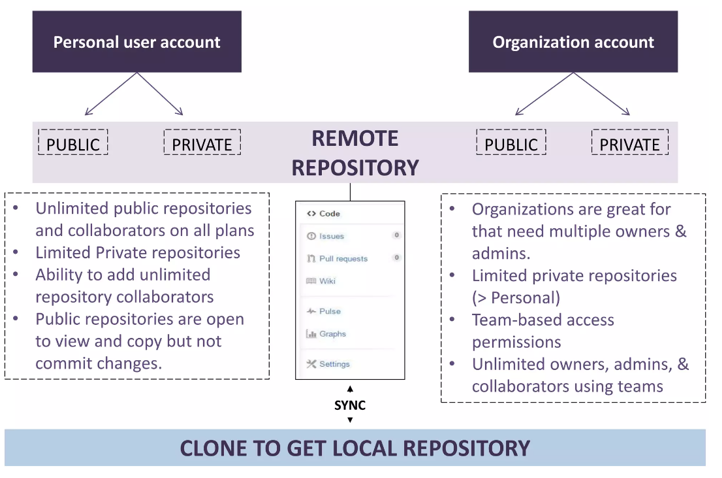
\includegraphics[width=0.6\linewidth]{githubstructure.PNG}
\end{figure}
    
\end{frame}

\begin{frame}{Flujo de trabajo en GitHub}

\begin{figure}
    \centering
    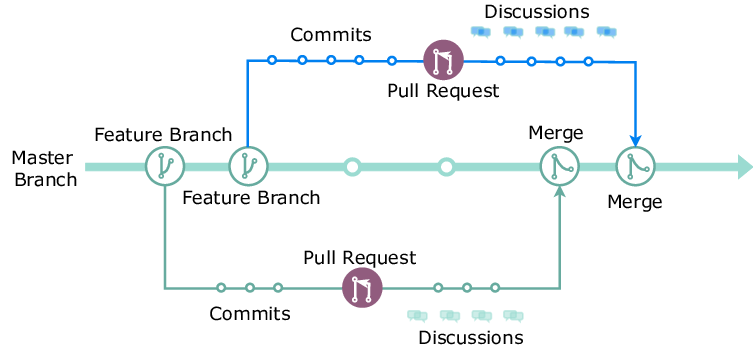
\includegraphics[width=0.5\linewidth]{workflow.png}
\end{figure}

Ejemplo: \url{https://github.com/jgrapht/jgrapht/pull/811}
    
\end{frame}

\section{Pipelines CI/CD}

\begin{frame}{Pipelines CI/CD}

\begin{block}{Pipeline}
    Una pipeline CI/CD es una secuencia automatizada de etapas que permiten construir, probar y entregar software de forma continua, rápida y fiable.
\end{block}

Fases típicas:

\begin{itemize}
    \item \textbf{Integración Continua.} Se centra en la automatización de la integración de cambios de código de diferentes desarrolladores en un repositorio compartido. Cada cambio se prueba automáticamente para garantizar que no introduce errores.

    \item \textbf{Entrega Continua.} Extiende la Integración Continua para que cada versión que supera las pruebas pueda ser puesta en producción en cualquier momento.
Esto se logra a través de una automatización del proceso de despliegue.

    \item \textbf{Despligue continuo.} Extiende a la Entrega Continua en que la puesta en producción se hace automáticamente y no manualmente.




\end{itemize}
    
\end{frame}

\begin{frame}{Pipelines CI/CD}

\begin{table}[h]
\centering
\scalebox{0.7}{
\begin{tabular}{|l|p{6cm}|c|}
    \hline
    \textbf{Práctica} & \textbf{¿Qué automatiza?} & \textbf{¿Llega a producción?} \\
    \hline
    Integración continua & Compilación + tests al hacer commit & ❌ No \\
    \hline
    Entrega continua     & CI + empaquetado (+ despliegue a \textit{staging}) &  Lista para producción (manual) \\
    \hline
    Despliegue continuo  & Entrega continua + despliegue automático &  Automáticamente \\
    \hline
\end{tabular}
}
\end{table}


    
\end{frame}




\begin{frame}{Pipelines CI/CD}

{\scriptsize
Integración continua:

\begin{itemize}
    \item Detección de cambios: trigger por push o pull request.

\item Checkout del código: clonar la rama actual.

 \item Compilación / build: generar binarios o artefactos.

\item Ejecución de tests automáticos: unitarios, integración, linting, etc.

\item Informe de resultados: fallos o aprobaciones (feedback rápido al equipo).
\end{itemize}

\pause

Entrega continua, lo anterior +:

\begin{itemize}
    \item Empaquetado del software: generar .jar, imagen Docker, zip, etc.
    \item Ejecución de tests adicionales: integración, aceptación, e2e.

\item Publicación en repositorio intermedio: Sonatype, Artifactory, Docker Hub (no necesariamente en producción).

\item Despliegue en entorno de staging / preproducción: para validación manual o QA.

\item Aprobación manual opcional: un responsable revisa antes de pasar a producción.
\end{itemize}
\pause

Despliegue continuo, lo anterior (sin la aprobación manual) +:

\begin{itemize}
    \item Despliegue automático en producción.
    \item Verificación y monitorización post-despliegue.
    \item Rollback automático si falla.
\end{itemize}


}


    
\end{frame}

\begin{frame}{Pipelines CI/CD}

Herramientas para definir pipelines:

\begin{figure}
    \centering
    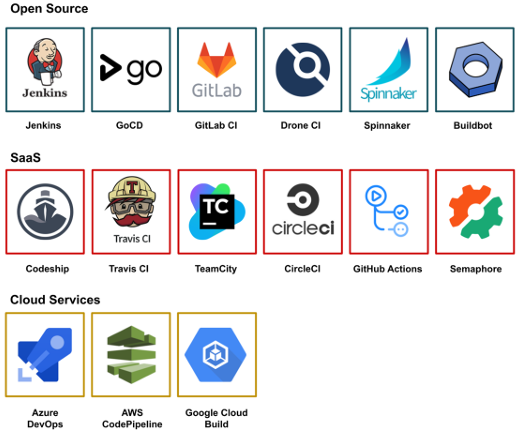
\includegraphics[width=0.5\linewidth]{toolscicd.PNG}
\end{figure}
    
\end{frame}


\section{GitHub Actions}

\begin{frame}{GitHub Actions}

\begin{block}{GitHub Actions}
GitHub Actions es una plataforma de integración y entrega continuas que te permite automatizar tu flujo de trabajo de compilación, prueba e implementación.
\end{block}

\begin{itemize}
    \item Se pueden crear \textit{workflows} que generen y prueben cada \textit{pull request} del repositorio, o mandar \textit{pull requests} fusionadas a producción
    \item GitHub Actions realmente va más allá de CI/CD, se pueden generar \textit{workflows} que reaccionen a distintos eventos del repositorio: por ejemplo, etiquetar un \textit{issue} cuando se genera
    \item GitHub Actions ofrece MVs Linux, Windows y macOS para ejecutar \textit{workflows}
\end{itemize}
    
\end{frame}

\begin{frame}{GitHub Actions}

\begin{block}{Componentes principales}

\begin{itemize}
    \item Un \textit{workflow} se activa cuando ocurre un evento del repositorio, como por ejemplo cuando se abre una \textit{pull request} o se crea una \textit{issue}.
    \item Un \textit{workflow} contiene uno o más \textit{jobs}, que pueden ejecutarse de forma secuencial o en paralelo.
    \item Cada \textit{job} se ejecutará dentro de su propia máquina virtual (\textit{runner}) y consta de uno o más \textit{steps}. Cada \textit{step} es una \textit{action} o un \textit{script}.
\end{itemize}

\end{block}

\begin{figure}
    \centering
    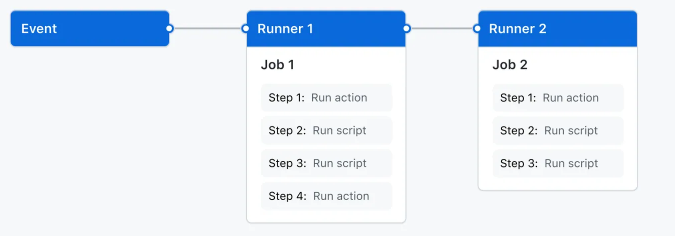
\includegraphics[width=0.5\linewidth]{actions.png}
\end{figure}
    
\end{frame}

\begin{frame}[fragile]{GitHub Actions}
\begin{itemize}
    \item Los workflows se definen en un YAML en la carpeta \texttt{.github/workflows/} 
\end{itemize}

\begin{minted}[fontsize=\tiny]{yaml}
# .github/workflows/ci.yml
name: CI

on:
  push:
    branches: [ "main" ]
  pull_request:
    branches: [ "main" ]

jobs:
  build:
    runs-on: ubuntu-latest

    steps:
    - name: Checkout repository
      uses: actions/checkout@v4

    - name: Set up JDK 17
      uses: actions/setup-java@v4
      with:
        java-version: '17'
        distribution: 'temurin'
        cache: maven

    - name: Build with Maven
      run: mvn -B clean verify
\end{minted}
\end{frame}

\begin{frame}{GitHub Actions}

\begin{itemize}
    \item El workflow se ejecuta al recibir un push a main o al abrir un pull request
    \item El workflow contiene un job que ejecuta tres steps
    \item El primer step es una acción predefinida que clona el repositorio
    \item El segundo step es una acción que instala JDK en la MV
    \item El último step es un script que ejecuta los tests
    \item El workflow anterior es para CI. Para tener entrega continua/despliegue continuo habría que añadir más pasos

\end{itemize}
    
\end{frame}

\section{Jenkins}

\begin{frame}{Jenkins}

\begin{block}{Jenkins}
Jenkins es una herramienta OS de CI/CD muy popular, escrita en Java, que permite automatizar el proceso de desarrollo, prueba e implementación de software.
\end{block}

\begin{itemize}
    \item Open source y gratuito

    \item Extensible mediante plugins (más de 1.800 disponibles para Git, Docker, Kubernetes, Maven, etc.)

    \item  Integración con la mayoría de herramientas DevOps (GitHub, GitLab, Bitbucket, SonarQube, etc.)
    
    \item Configuración declarativa (por ejemplo, usando Jenkinsfile para definir pipelines en código)
    
    \item Escalabilidad con nodos/agentes: se puede distribuir la carga de trabajo en varios servidores
\end{itemize}
    
\end{frame}

\begin{frame}{Jenkins: conceptos principales}

{\scriptsize

\begin{itemize}
    \item Un \textit{pipeline} de Jenkins se ejecuta cuando ocurre un evento configurado, como un commit, una compilación manual o una ejecución programada.

    \pause
    
    \item Cada ejecución concreta del \textit{pipeline} se denomina \textit{build}. Jenkins asigna un número único a cada \textit{build} y almacena sus registros, artefactos y estado (éxito, fallo, abortado).

    \pause
    
    \item Un \textit{pipeline} se compone de uno o más \textit{stages}, que representan las fases principales del proceso (por ejemplo, \textit{Build}, \textit{Test}, \textit{Deploy}).

    \pause
    
    \item Cada \textit{stage} contiene varios \textit{steps}, que son las instrucciones individuales que Jenkins ejecuta (por ejemplo, ejecutar un comando \texttt{sh}, clonar un repositorio o invocar una herramienta externa).

    \pause 
    
    \item Los \textit{steps} se ejecutan dentro de un entorno de agente (\textit{agent}), que puede ser el nodo principal (\textit{controller}) o un nodo remoto (\textit{agent}) configurado para la ejecución.

    \pause
    \item Cada \textit{build} se ejecuta en un \textit{workspace}, es decir, un directorio aislado en el agente donde Jenkins descarga el código fuente, ejecuta los \textit{steps} y guarda los artefactos generados.

    \pause
    
    \item Jenkins permite definir los \textit{pipelines} mediante un archivo \texttt{Jenkinsfile}.
\end{itemize}

}
    
\end{frame}

\begin{frame}{Jenkins vs GitHub Actions}

\begin{table}[h!]
\centering
\scalebox{0.5}{
\begin{tabular}{|p{3.5cm}|p{5cm}|p{5cm}|}
\hline
\rowcolor{gray!15}
\textbf{Concepto} & \textbf{GitHub Actions} & \textbf{Jenkins} \\ 
\hline
Definición del flujo de CI/CD &
\texttt{.github/workflows/*.yml} &
\texttt{Jenkinsfile}  \\ 
\hline
Unidad principal de ejecución &
\textit{Workflow} &
\textit{Pipeline} \\ 
\hline
Ejecución individual del flujo &
\textit{Run} &
\textit{Build} \\ 
\hline
Bloques de trabajo dentro del flujo &
\textit{Job} &
\textit{Stage} \\ 
\hline
Pasos dentro de un bloque &
\textit{Step} &
\textit{Step} (idéntico concepto) \\ 
\hline
Acción o tarea reutilizable &
\textit{Action} (de GitHub Marketplace o propia) &
\textit{Shared Library} o \textit{Step plugin} \\ 
\hline
Entorno de ejecución &
\textit{Runner} (GitHub-hosted o self-hosted) &
\textit{Agent} (controller o nodo remoto) \\ 
\hline
Espacio de trabajo temporal &
\texttt{\$\{GITHUB\_WORKSPACE\}} &
\texttt{\$\{WORKSPACE\}} \\ 
\hline
Evento que dispara la ejecución &
\textit{Trigger event} (\texttt{push}, \texttt{pull\_request}, etc.) &
\textit{Trigger} (manual, commit, etc.) \\ 
\hline
Resultado de ejecución &
\textit{Status} (\texttt{success}, \texttt{failure}, \texttt{cancelled}) &
\textit{Build result} (\texttt{SUCCESS}, \texttt{FAILURE}, \texttt{ABORTED}) \\ 
\hline
\end{tabular}}
\caption{Equivalencia aproximada de términos entre GitHub Actions y Jenkins}
\end{table}

    
\end{frame}

\begin{frame}[fragile]{Jenkins: Jenkinsfile}

\begin{minted}[fontsize=\scriptsize]{python}
pipeline {
    agent {
        docker {
            image 'maven:3.9.6-eclipse-temurin-17'
            label 'docker-node'
        }
    }

    stages {
        stage('Checkout') {
            steps {
                checkout scm
            }
        }

        stage('Build with Maven') {
            steps {
                sh 'mvn -B clean verify'
            }
        }
    }
}

\end{minted}
    
\end{frame}

\begin{frame}{Jenkins: Jenkinsfile}

\begin{itemize}
    \item Se hace uso del plugin de Docker
    \item Esto se va a ejecutar en un contenedor dentro de una máquina agente
    \item Primero se hace un checkout (clone del repositorio)
    \item Finalmente se ejecutan los scripts
    \item Si se quiere ejecutar directamente en la máquina agente, habría que instalar en dicho agente maven y JDK (se puede instalar añadiendo una \textit{stage set-up} o mediante la interfaz gráfica)
    \item En este caso un único agente ejecuta todos los steps. Pero se puede especificar que cada step lo haga un agente diferente.
\end{itemize}
    
\end{frame}


\begin{frame}{Jenkins: arquitectura}

Jenkins sigue una arquitectura maestro-esclavo:

\begin{itemize}
    \item \textbf{Controller (\textit{Master})}
    \begin{itemize}
        \item Coordina la ejecución de las \textit{pipelines}.
        \item Proporciona la interfaz web y gestiona los \textit{plugins}, la configuración y la cola de builds.
        \item Decide qué \textit{agent} ejecutará cada trabajo.
    \end{itemize}

\pause
    \item \textbf{Agents (\textit{Slaves})}
    \begin{itemize}
        \item Son los nodos que ejecutan los \textit{jobs} y \textit{steps} enviados por el controller.
        \item Cada agente dispone de su propio \textit{workspace}, herramientas y sistema operativo.
        \item Ejemplos de agentes:
        \begin{itemize}
            \item \textbf{Agent Linux:} Maven 3.9, JDK 17.
            \item \textbf{Agent Windows 10:} PowerShell, .NET SDK.
        \end{itemize}
    \end{itemize}

    \pause

    \item \textbf{Comunicación}
    \begin{itemize}
        \item El controller envía las tareas a los agentes a través de un canal seguro (SSH, JNLP, WebSocket).
        \item Los agentes ejecutan las builds y devuelven logs y artefactos al controller.
    \end{itemize}
\end{itemize}



    
\end{frame}




\end{document}